% 原文 pp.181–187（印刷 pp.1299–1305）
% Lecture 13：$\mathcal{N}=2$ 二维超对称理论（一），第二部分（§13.4–§13.5）

% ===== 原文 p.181 =====
我们如下选取各 $R$ 对称群在以 $A_i$、$P$ 为截面的线丛上的作用：以 $A_i$ 为截面的线丛 $L_i$ 在各 $R$ 对称性下不变；而以 $P$ 为截面的线丛 $L_{n+1}$ 在由空间转动诱导出的 $R$ 对称性下不变，并且在来自四维空间 $R$ 对称性的那个 $R$ 对称性下具有权二。作了这样的 $R$ 对称作用选择之后，任何形如
\[
  W=P\cdot F(A_i)
\]
的超势（其中 $F$ 是 $A_1,\dots,A_n$ 的任意多项式）都在各 $R$ 对称性下不变。当然还有一个附加条件，即 $W$ 必须是规范不变的。这意味着 $F$ 必须是 $n$ 次齐次多项式。于是，任何这种形式的 $W$ 都会在拉氏量中给出一个规范不变、并且在 $R$ 对称性下不变的项。这就是具有这些对称性的最一般的相互作用。

\subsection{经典分析}
% 原文 §13.4.1

既然已经把理论详细确定下来，我们便想弄清它究竟是什么，特别是在 $r\to\pm\infty$ 的极限下。我们先作经典分析。把拉氏量中出现的每一个超场写成其分量形式
\begin{align*}
  A &= a+\theta(\cdots)+\cdots,\\
  P &= p+\theta(\cdots)+\cdots,\\
  \Sigma &= \sigma+\theta(\cdots)+\cdots.
\end{align*}
超场 $\Sigma$ 包含辅助场 $D$ 与 $F$，它们可以用各自的运动方程消去。

玻色势是这些场的玻色分量的函数 $V(a,p,\sigma)$。对于我们已描述的这个拉氏量，势取如下形式
\begin{equation}
  \tag{13.3}
  \label{eq:13-3}
  V(a,p,\sigma)=\frac{1}{2e^{2}}D^{2}+|dW|^{2}+|\sigma|^{2}\Bigl(\sum|a_i|^{2}+n^{2}|p|^{2}\Bigr).
\end{equation}
方程 (13.3) 中最后一项的来源如下：在四维中，一个手征场 $\Phi=\phi+\theta(\cdots)+\cdots$ 会在势中导致一项
\[
  \sum_{\mu=0}^{3}\left|\frac{D\phi}{Dx^{\mu}}\right|^{2},
\]
当它约化到二维时变成
\[
  \sum_{\alpha=0}^{1}\left|\frac{D\phi}{Dx^{\alpha}}\right|^{2}+n^{2}|\sigma|^{2}|\phi|^{2},
\]
这里 $\phi$ 的电荷为 $n$。

% [Tutor Note: (13.3) 中的 $D$ 是\emph{尚未}被消去的辅助场，所以势里出现的是 $\frac{1}{2e^{2}}D^{2}$；而 (13.4) 给出的 $D=\sum|a_i|^{2}-n|p|^{2}-r$ 其实是矩映射的取值，二者相差一个 $e^{2}$ 因子。正确的记账是：把运动方程 $D=-e^{2}\bigl(\sum q_i|\phi_i|^{2}-r\bigr)$ 代回，才得到 p.185 上消去后的形式 $\frac{e^{2}}{2}\bigl(\sum|A_i|^{2}-n|P|^{2}-r\bigr)^{2}$，以及 $a=p=0$ 时的常数项 $V_{\mathrm{eff}}=\frac{e^{2}}{2}r^{2}$（(13.6)）。若把 (13.3) 中的 $D$ 直接用 (13.4) 的矩映射值代入而写成 $\frac{1}{2e^{2}}\bigl(\cdots\bigr)^{2}$，结果会与 (13.6)、p.185 相差 $e^{4}$——这是本讲最容易出的耦合常数记账错误。另需注意：$V=0$ 要求 $D=0$，正是因为 (13.3) 写的是消去前的形式。]

% [Tutor Note: (13.3) 末项的系数 $n^{2}$ 来自四维约化：四维手征场动能项 $\sum_{\mu=0}^{3}|D_\mu\phi|^{2}$ 中 $\mu=3$ 的分量经 $A_3\to\sigma$ 化为 $|(\partial_3-inA_3)\phi|^{2}\to n^{2}|\sigma|^{2}|\phi|^{2}$，故系数是电荷的\emph{平方}；而 (13.4) 中 $P$ 的贡献是线性的 $-n|p|^{2}$，因为矩映射对每个场是线性的。把这两处的 $n$ 与 $n^{2}$ 弄混是常见错误。还须记住：此处的 $\sigma$ 是矢量多重态中的标量（即约化后的 $A_3$），不是 Higgs 场，它的期望值不破缺规范对称性，却给带电场提供质量。]

一般来说，“$D$ 项”（即 $\Sigma$ 中的辅助场）按其运动方程等于 $\sum q_i|\phi_i|^{2}-r$。这在数学上其实是一个熟悉的对象；它正是生成平坦 Kähler 流形（$\mathbb{C}^{s}$ 的一份拷贝，$s$ 为手征超场的个数）上 $U(1)$ 规范作用的“矩函数”（moment function），而手征超场正是在这个流形中取值的。在我们的例子里，它成为
\begin{equation}
  \tag{13.4}
  \label{eq:13-4}
  D=\sum|a_i|^{2}-n|p|^{2}-r.
\end{equation}
由于 $W=P\cdot F(A)$，我们还有
\begin{equation}
  \tag{13.5}
  \label{eq:13-5}
  |dW|^{2}=|F|^{2}+|p|^{2}|dF|^{2}.
\end{equation}

% ===== 原文 p.182 =====
我们将集中讨论 $F$ 是横截的（transverse）情形，即 $F=dF=0$ 只在原点成立。

我们要找出所有的经典零能解，换言之，求解 $V=0$。由于势的形式，这要求 (i) $D=0$，(ii) $|dW|^{2}=0$，以及 (iii) 或者 $\sigma=0$，或者 $\sum|a_i|^{2}+n^{2}|p|^{2}=0$。此外我们还需要把 $U(1)$ 下的规范等价考虑进来。

首先注意，由 (13.5)，当 $p\ne0$ 时令 $|dW|^{2}=0$ 便推出 $F=dF=0$，于是按横截性条件所有 $a_i=0$。因此只有两种情形：$p=0$，或者对一切 $i$ 都有 $a_i=0$。另一方面，若 $r\ne0$，则由 (13.4) 并注意 $D=0$，$p=0$ 与“一切 $a_i=0$”不能同时成立。（事实上 $r$ 的符号将决定这两者中哪一个成立。）因此当 $r\ne0$ 时 $\sum|a_i|^{2}+n^{2}|p|^{2}\ne0$，从而 $\sigma$ 必须为零。

% [Tutor Note: 从 (13.5) 到“只有两种情形”之间作者跳了一步，补出来是：若 $p\ne0$ 而 $|dW|^{2}=0$，则 $|F|^{2}+|p|^{2}|dF|^{2}=0$ 的两项分别非负，只能各自为零，即在 $a_i$ 处 $F=0$ 且 $dF=0$，再由横截性得 $a_i=0$；反之若 $p=0$，则 $|dW|^{2}=0$ 只要求 $F(a)=0$，$a_i$ 可以非零。第二步：$D=0$ 且 $p=0$ 时 (13.4) 给出 $\sum|a_i|^{2}=r$，故只在 $r>0$ 时有解；$D=0$ 且 $a_i=0$ 时给出 $n|p|^{2}=-r$，故只在 $r<0$ 时有解；$r=0$ 时两种情形都退化到原点，这正是 p.185 所述奇点之所在。第三步（原文的 (iii)）：$|\sigma|^{2}$ 的系数 $\sum|a_i|^{2}+n^{2}|p|^{2}$ 非负，故 $V=0$ 迫使它为零；当该括号非零时只能 $\sigma=0$。三处逻辑缺环都在此补全。]

现在考虑 $r>0$ 的情形。经典真空的方程成为 $p=0$、$\sum|a_i|^{2}=r$、$F=0$，而且我们必须对规范群 $U(1)$ 的作用取商。这给出 $\mathbb{CP}^{n-1}$ 中由方程 $F=0$ 定义的超曲面 $X$，其 Kähler 类为 $r$。于是经典地，我们的理论可以描述为一个非线性 $\sigma$ 模型，其目标空间就是这个超曲面 $X$，所用的度量的 Kähler 类之体积正比于 $r^{n-2}$。正如上面已指出的，这样的理论中心荷为 $\hat c=n-2$。

% [Tutor Note: 这里的 $\hat c=n-2$ 用的是 $\hat c=c/3$ 的约定（二维 $\mathcal{N}=2$ 超共形代数的中心荷通常记作 $\hat c$）。超曲面 $X\subset\mathbb{CP}^{n-1}$ 的复维数正是 $n-2$，而 Calabi–Yau $d$ 重态上的非线性 $\sigma$ 模型满足 $c=3d$、即 $\hat c=d$。所以“$\hat c=n-2$”与“$\dim_{\mathbb{C}}X=n-2$”是同一句话；若误读成 $c=n-2$，就会与五重超曲面（$n=5$ 时 $c=9$、$\hat c=3$）的熟知结果矛盾。同理，p.183 上单场 $A^{n}$ 超势的 $\hat c=\frac{n-2}{n}=1-\frac{2}{n}$ 正是 $\mathcal{N}=2$ 极小模型系列 $\hat c=1-\frac{2}{k}$ 的成员，而 $n\cdot\frac{n-2}{n}=n-2$ 才与几何一侧相符——这两处的一致性正是下文论证的骨架。]

这一经典描述在 $r\gg0$ 时是对量子理论的良好近似，因为在那里非线性 $\sigma$ 模型是弱耦合的。事实上，由于非线性 $\sigma$ 模型是稳定的（即没有相关微扰），而边际微扰只会改变复化 Kähler 结构与复结构，我们应当预期我们的量子理论与这一族 $\sigma$ 模型中的某一个成员相重合。

另一方面，当 $r<0$ 时，经典真空的空间满足 $a_i=0$ 与 $n|p|^{2}=-r$。我们可以用规范变换把 $p$ 固定为 $\sqrt{-r/n}$，从而留下 $\mathbf{Z}_n$ 的剩余规范不变性，也就是说，原来的 $U(1)$ 规范群破缺为 $\mathbf{Z}_n$。因此这将是一个所谓的“轨形”（orbifold）理论，其中 $\mathbf{Z}_n$ 会在理论的整体分析中出现（其出现方式我们稍后描述）。理论的局域描述（对此可以忽略轨形化问题）是这样的：当 $r\ll0$ 时，场 $P$ 有很大的质量，可以被积掉，留下 $n$ 个无质量手征超场 $A_1,\dots,A_n$ 的有效理论，其有效相互作用为
\[
  W_{\mathrm{eff}}=\text{常数}\cdot F(A_1,\dots,A_n),
\]
其中 $F$ 是 $n$ 次齐次多项式。

这种由 $n$ 个无质量场加上一个多项式相互作用构成的理论称为 Landau–Ginzburg 理论。它显然应当在红外（IR）流向一个中心荷为 $\hat c=n-2$ 的共形场论。我们预期如此，因为那正是 $r\gg0$ 时的取值。按 Zamolodchikov $c$ 定理（见本讲末尾所列的参考文献），$c$ 在一族共形场论中是常数；因此只要对所有 $t$ 都存在流向共形场论的流动，$r\to+\infty$ 与 $r\to-\infty$ 就应给出同一个值。

% [Tutor Note: 作者两次援引 Zamolodchikov $c$ 定理，但用法是“反用”的：$c$ 定理说的是 $c$ 沿重整化群流单调下降、且在不动点处驻定，因此若两个端点都是共形场论而中间存在非平凡流动，则必有 $c_{\mathrm{IR}}<c_{\mathrm{UV}}$。此处的 $r$（即 $t$ 的实部）只是一个\emph{边际}参数，改变它并不产生流动，理论对所有 $t$ 都停留在同一族共形场论上，故 $c$ 与 $t$ 无关。原文“若对所有 $t$ 都存在流向共形场论的流动”这一条件，隐含的正是“没有相关微扰、流动是平凡的”；严格论证须验证 $F$ 的横截性确实排除了相关算符（详见 Witten 关于 $\mathcal{N}=2$ 极小模型的 Landau–Ginzburg 描述一文，以及 Vafa 关于轨形化 Landau–Ginzburg 模型的工作）。]

让我们检验这个预言。仍由 Zamolodchikov 定理，$F$ 的选择应当无关紧要，所以我们考虑一个特殊的选择，即“Fermat 型”的 $F$：
\[
  F(A_1,\dots,A_n)=\sum_i A_i^{n}.
\]
具有这种相互作用的 Landau–Ginzburg 理论将（至少在局域上）分解为 $n$ 个相同理论的乘积，每个理论只含一个手征超场 $A$，其超势为

% ===== 原文 p.183 =====
$A^{n}$。我们的预言意味着这些理论中每一个的中心荷都必须是 $\hat c=\frac{n-2}{n}$。而这恰好就是极小模型（minimal model）的中心荷！所以，只要我们能把极小模型与这个 Landau–Ginzburg 理论等同起来，就建立了这一结果。（同时我们也会得知：具有 Fermat 型超势的 Landau–Ginzburg 模型是代数可解的。）我们将在第 15 讲回到这个问题。请注意：如果我们得到的 $\hat c$ 值小于一、且不具有 $1-2/k$（$k$ 为某个整数）的形式，我们就会陷入困境！

\subsection{轨形化}
% 原文 §13.4.2

正如上面指出的，当 $r\ll0$ 时，我们理论原来的 $U(1)$ 规范对称群在有效理论中被破缺为 $\mathbf{Z}_n$。因此，如果考虑低能有效理论在 Riemann 面 $\Sigma$ 上的路径积分，$U(1)$ 规范群就约化为 $\mathbf{Z}_n$，我们只需对所有平坦的 $\mathbf{Z}_n$ 丛求和。在任何曲面 $\Sigma$ 上，一个平坦 $\mathbf{Z}_n$ 丛可以由它绕 $\Sigma$ 中各条圈的和乐 $\gamma_1,\dots,\gamma_k\in\mathbf{Z}_n$ 来指定。在具有 $\mathbf{Z}_n$ 对称性的理论中对所有平坦 $\mathbf{Z}_n$ 丛求和，这一手续称为对该理论作轨形化（orbifolding）。

在（表述于圆 $S^{1}$ 上的）Hamilton 表述中，我们需要把绕该圆的和乐 $\gamma\in\mathbf{Z}_n$ 作为确定一个态的数据的一部分。设 $\mathcal{H}_\gamma$ 为和乐为 $\gamma$ 的态所构成的 Hilbert 空间。（于是，带有边界、且边界上已指定平坦 $\mathbf{Z}_n$ 丛的 Riemann 面，将决定在这些不同的 Hilbert 空间之间映照的算符，具体取决于边界圈上的和乐。）$\mathbf{Z}_n$ 作用在每个 $\mathcal{H}_\gamma$ 上：由于群 $\mathbf{Z}_n$ 是阿贝尔的，绕圆一周时用 $\mathbf{Z}_n$ 的某个元素作扭曲，是与 $\mathbf{Z}_n$ 对易的操作。

我们断言，轨形化理论的 Hilbert 空间是
\[
  \mathcal{H}=\bigoplus_{\gamma}\bigl(\mathcal{H}_\gamma\bigr)^{\mathbf{Z}_n}.
\]
为看清这一点，考虑两端和乐为 $\gamma$ 的柱面：

\begin{figure}[htbp]
  \centering
  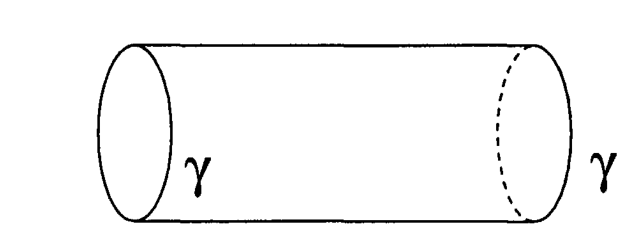
\includegraphics[width=0.42\textwidth]{figs/fig_p183_1.png}
  \caption{两端和乐均为 $\gamma$ 的柱面；右端的虚线表示远端的边界圈。（原文 Figure 1，p.183）}
  \label{fig:p183-1}
\end{figure}

% [Tutor Note: 这里的双重手续容易混淆：先固定边界上的和乐 $\gamma$ 得到扭曲扇区 $\mathcal{H}_\gamma$，再对残余的 $\mathbf{Z}_n$ 取不变子空间。$\mathbf{Z}_n$ 在 $\mathcal{H}_\gamma$ 上的作用来自绕空间圆的大规范变换；正因为 $\mathbf{Z}_n$ 阿贝尔，沿时间方向的扭曲 $\gamma'$ 与沿空间方向的 $\gamma$ 可以对易，$\gamma'$ 才能在 $\mathcal{H}_\gamma$ 上有良好定义并取迹。若群非阿贝尔，$\gamma'$ 一般不再把 $\mathcal{H}_\gamma$ 映到自身，必须按共轭类重组扇区——那是非阿贝尔轨形化的额外结构，本讲的论证不适用。]

如我们已经注意到的，$\mathbf{Z}_n$ 在每个扇区 $\mathcal{H}_\gamma$ 上仍有作用；设 $\gamma'\in\mathbf{Z}_n$ 决定一个算符 $\gamma':\mathcal{H}_\gamma\to\mathcal{H}_\gamma$。这个算符的迹可以作为一个环面上的配分函数 $Z_{\gamma'\gamma}$ 来计算：

\begin{figure}[htbp]
  \centering
  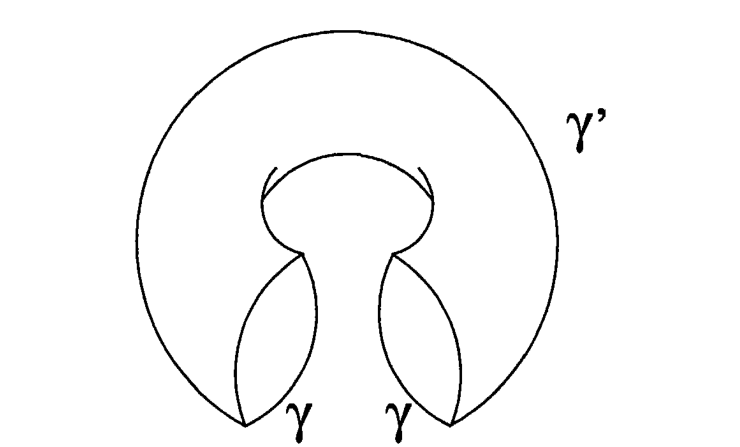
\includegraphics[width=0.46\textwidth]{figs/fig_p183_2.png}
  \caption{在环面上计算 $\mathrm{Tr}_{\mathcal{H}_\gamma}\gamma'q^{H}$：外侧大圈标以 $\gamma'$，底部两个小圈标以 $\gamma$，表示两个方向上分别作 $\gamma'$ 与 $\gamma$ 的扭曲。（原文 Figure 2，p.183）}
  \label{fig:p183-2}
\end{figure}

% ===== 原文 p.184 =====
它是用 $\gamma'$ 去扭曲柱面边界圈上丛的认同（identification）而构造的，即
\[
  Z_{\gamma'\gamma}=\mathrm{Tr}_{\mathcal{H}_\gamma}\,\gamma'\,q^{H}.
\]
更内蕴地说，在这个环面上，一个方向上有 $\gamma$ 的扭曲，另一个方向上有 $\gamma'$ 的扭曲，如图所示。

如果把各算符 $\gamma'$ 求和，结果便是 $n\pi$，其中 $\pi$ 是到 $\mathbf{Z}_n$ 不变子空间上的投影：
\[
  \frac{1}{n}\sum_{\gamma'}Z_{\gamma'\gamma}
  =\mathrm{Tr}_{\mathcal{H}_\gamma}\,\pi\,q^{H}
  =\mathrm{Tr}_{(\mathcal{H}_\gamma)^{\mathbf{Z}_n}}\,q^{H}.
\]
现在，$\mathbf{Z}_n$ 规范理论的配分函数可由下述方式得到：把亏格一的配分函数对所有方向上的一切可能扭曲求和，并（由于我马上要说明的理由）除以 $n$。这给出
\[
  \frac{1}{n}\sum_{\gamma,\gamma'}Z_{\gamma'\gamma}
  =\mathrm{Tr}_{\oplus_\gamma(\mathcal{H}_\gamma)^{\mathbf{Z}_n}}\,q^{H},
\]
由此我们断定，我们问题的 Hilbert 空间确实就是 $\mathcal{H}=\bigoplus_\gamma(\mathcal{H}_\gamma)^{\mathbf{Z}_n}$。

% [Tutor Note: $\sum_{\gamma'}\gamma'=n\pi$ 是有限群上的标准平均：在 $\mathbf{Z}_n$ 的正则表示中，非单位元素的特征标之和为零，故求和恰为 $|G|$ 倍到不变子空间的投影算符（等价地，$\frac1n\sum_{\gamma'}\gamma'$ 是投影）。随后出现的两个 $n$ 容易混淆：第一个 $1/n$ 来自对扭曲 $\gamma'$ 的平均，第二个 $1/n$（在 $\frac1n\sum_{\gamma,\gamma'}$ 中）来自除以规范群体积 $|G|=n$。二者数值相同而来源不同；漏掉任何一个都会使配分函数整体差一个 $n$ 的因子，从而把 Hilbert 空间的维数算错。]

或许我应当解释一下，为什么
\[
  Z=\frac{1}{n}\sum_{\gamma,\gamma'}Z_{\gamma'\gamma}
\]
才是 $\mathbf{Z}_n$ 规范理论合适的配分函数。在规范理论中作路径积分时，人们应当对联络求和并除以规范群的体积。当规范群是正维数的 Lie 群时，联络的空间是无穷维的。规范变换群同样是无穷维的，而要使“除以规范群的体积”这句话有意义，就需要 Faddeev–Popov 构造并引入鬼场。在目前的情形中，我们考虑的是规范群为 $\mathbf{Z}_n$ 的低能有效理论。$\Sigma$ 上仅有的联络就是取值于 $\mathbf{Z}_n$ 的平坦联络。所以对 $\gamma$ 与 $\gamma'$ 的求和就是关于联络的路径积分。$\Sigma$ 上仅有的规范变换是由 $\mathbf{Z}_n$ 的元素所作的常值变换；因此规范群的体积就是 $n$，即规范群元素的个数。于是“除以规范群的体积”就由除以 $n$ 来实现。

\subsection{从正 $r$ 到负 $r$ 的插值}
% 原文 §13.4.3

我们的经典分析可以总结如下：我们需要令 $D=dW=0$，并除以 $U(1)$。令 $D=0$ 并除以 $U(1)$ 这一步，就是数学上熟悉的辛约化（symplectic reduction）操作，其中 $D=0$ 定义了 $U(1)$ 作用的矩映射的一个水平集（$r$ 的选取指定了该水平）。这一过程还有另一种数学解释，即几何不变量理论（Geometric Invariant Theory，GIT）意义下的商：我们把群 $U(1)$ 复化为 $\mathbb{C}^{*}$，并考虑 $\mathbb{C}^{*}$ 以与前面相同的权在 $\mathbb{C}^{n+1}$ 上的作用（$A_i$ 的权为 $1$，$P$ 的权为 $-n$）。在这个具体例子中存在两种可能的 GIT 商（它们实际上拓扑不同）：当 $r>0$ 时，该商可以解释为丛 $\mathcal{O}_{\mathbf{P}^{n-1}}(-n)$ 的全空间（其中 $p$ 充当纤维坐标），而当 $r<0$ 时，该商是 $\mathbb{C}^{n}/\mathbf{Z}_n$。

% ===== 原文 p.185 =====
在两种情形下我们都还必须施加 $dW=0$：在 $r>0$ 的情形，$W=PF(A_1,\dots,A_n)$ 是一个非退化函数（在 Bott 引入的广义意义下），而 $\mathcal{O}_{\mathbf{P}^{n-1}}(-n)$ 中临界点的集合就是 $\mathbf{P}^{n-1}$ 中由方程 $F=0$ 定义的那个簇；在 $r<0$ 的情形，我们有一个齐次多项式 $F(A_1,\dots,A_n)$，它在 $\mathbb{C}^{n}/\mathbf{Z}_n$ 的原点处有高度退化的临界点。

我们拉氏量中的自然参数是 $t=-ir+\frac{\theta}{2\pi}$。正是由于可以取 $\theta\ne0$，我们才能从正 $r$ 插值到负 $r$，而不遇到经典几何中会碰到的那个奇点。

\begin{figure}[htbp]
  \centering
  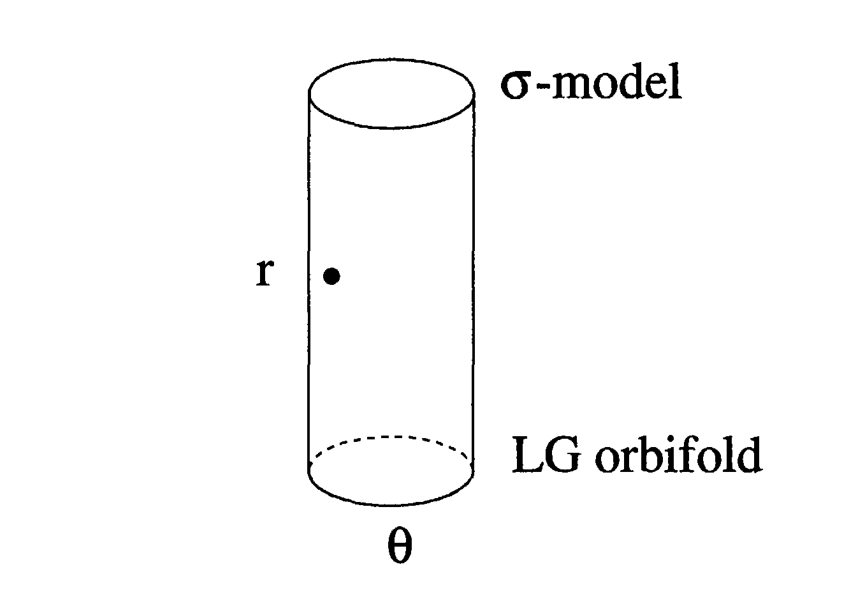
\includegraphics[width=0.40\textwidth]{figs/fig_p185_1.png}
  \caption{参数空间的柱面：竖直方向为 $r$，水平方向为 $\theta$，即复坐标 $t=-ir+\frac{\theta}{2\pi}$；上端 $r\gg0$ 处是 $\sigma$ 模型，下端 $r\ll0$ 处是 Landau–Ginzburg 轨形，柱面上的黑点标出 $r=0$ 处的奇点。（原文 Figure 3，p.185）}
  \label{fig:p185-1}
\end{figure}

经典地，在任意 $\theta$ 下 $r=0$ 处都有奇点，因而插值是不可能的。量子力学地，我们断言这个奇点将是孤立的，位于 $r=r_0$（对某个 $r_0$）且 $\theta=0$。（经典地奇点在 $r=0$；但量子力学地，它被一个我们即将讨论的单圈修正从 $r=0$ 移开了。）人们相信没有别的奇点；我们不会严格证明这一断言，而只解释物理学家相信它为真的一些理由。我们分析中较严格的部分，将是论证在这个位置确实存在奇点；较不严格的部分，则是论证这是唯一的奇点。

为作这一论证，我们再次把空间取为半径有限的圆 $S^{1}$。紧致性意味着情况与零空间维数中的普通量子力学颇为相似，所以我们先回顾一下质点普通量子力学中会发生什么。设粒子在流形 $X$ 上运动，势函数为 $V$。如果 $X$ 紧致，或者 $V$ 在 $X$ 的“两端”增长，那么我们可以变动 $X$ 与 $V$ 所依赖的参数，而不遇到量子力学基态的奇点。然而，若把参数变到某一点，使得 $V$ 在无穷远处不再增长，就会得到奇点。例如，若 $X=\mathbf{R}$，$V=\frac12 kx^{2}$（$x$ 为 $\mathbf{R}$ 上的线性函数），则只要 $k>0$，基态波函数就是 $k$ 的光滑函数，但在 $k=0$ 处会出现奇点。$k=0$ 的问题没有可归一化的基态波函数。

在我们的圆上问题中也会发生类似的事情。回忆我们的势的形式是
\[
  V=|P|^{2}|F|^{2}+|dF|^{2}
  +\frac{e^{2}}{2}\Bigl(\sum|A_i|^{2}-n|P|^{2}-r\Bigr)^{2}
  +|\sigma|^{2}\Bigl(\sum|A_i|^{2}+n^{2}|P|^{2}\Bigr).
\]

% [Tutor Note: 上式前两项印作 $|P|^{2}|F|^{2}+|dF|^{2}$，与 (13.5) 的 $|dW|^{2}=|F|^{2}+|p|^{2}|dF|^{2}$ 不符，正确写法应为 $|F|^{2}+|P|^{2}|dF|^{2}$，即 $|P|^{2}$ 应当乘在 $|dF|^{2}$ 上。三条判据：(i) (13.5) 只是对 $W=PF(A)$ 求导的直接结果；(ii) p.182 的论证“$p\ne0$ 时 $|dW|^{2}=0\Rightarrow F=dF=0$”恰恰要求 $|F|^{2}$ 的系数为 $1$ 而不是 $|p|^{2}$，否则 $p\to0$ 时该项自动消失，横截性条件就用不上了；(iii) 只有当 $|P|$ 大时 $A_i$ 才获得 $|P|^{2}|dF|^{2}$ 型的大质量，这与 p.186 上“$A$、$P$ 很小时其质量量级为 $|\sigma|^{2}$”的讨论一致。故这是原书的排版笔误，译文按原文照录，并在正文外指出。]

对一般的 $r$，这个理论具有势在无穷远处增长的性质。这保证了理论有离散谱，且其基态波函数随参数光滑变化。然而在 $r=0$ 时我们看到，只要 $A_i$ 与 $P$ 趋于零，就可以在 $\sigma$ 方向走到无穷远而不付出能量代价。这提示

% ===== 原文 p.186 =====
在 $r=0$ 时可能存在连续谱，以及基态波函数的奇点。

为了更细致地研究这个问题，我们需要理解理论在危险区域（即 $\sigma$ 很大而其他场很小）中的行为。当 $A$ 与 $P$ 非常接近零、而 $\sigma$ 很大时，$A$ 与 $P$ 有很大的质量（量级为 $|\sigma|^{2}$），可以被积掉，留下一个纯规范理论，其有效玻色势在经典层面只是一个常数
\begin{equation}
  \tag{13.6}
  \label{eq:13-6}
  V_{\mathrm{eff}}=\frac{e^{2}}{2}r^{2}.
\end{equation}
如果这就是正确答案，那么能量小于 $e^{2}r^{2}/2$ 的量子态在 $\sigma$ 很大的区域中会指数衰减。若如此，这个区域只可能在 $r=0$ 时对零能的超对称基态构成危险——并导致这种态的波函数出现奇点。

为了更好理解这一情形，我们必须在量子层面作类似的论证。为此考虑 $\sigma$ 所属的那个超场，即写出
\[
  \Sigma=\sigma+\theta\lambda+\theta\bar\theta(F+iD).
\]
超对称规范理论的作用量为
\begin{equation}
  \tag{13.7}
  \label{eq:13-7}
  \frac{1}{2e^{2}}\int d^{4}\theta\,\bar\Sigma\Sigma
  +\Bigl(\int d\bar\theta^{+}\,d\theta^{-}\,t\Sigma+\text{c.c.}\Bigr).
\end{equation}
如果在有效拉氏量 (13.7) 中完成 $\theta$ 积分，我们得到
\[
  \frac{1}{e^{2}}\int d^{2}x\left(\frac{F^{2}}{2}+|d\sigma|^{2}+\bar\lambda\not{\partial}\lambda\right)
  +\int d^{2}x\left(\frac{e^{2}r^{2}}{2}\right)
  +i\theta\int_{\Sigma}\frac{F}{2\pi},
\]
其中既包含一个曲率项（乘以一个“$\theta$ 角”），也包含前面讨论过的玻色势。

% [Tutor Note: 注意 $\theta$ 积分前后系数的变化：作用量 (13.7) 中写的是 $\frac{1}{2e^{2}}\int d^{4}\theta\,\bar\Sigma\Sigma$，而积分后动能项前变成 $\frac{1}{e^{2}}$。具体数值因子取决于 $\theta$ 测度与 $\bar\Sigma\Sigma$ 展开的约定，不宜死记，可靠的核对办法是：只保留 $D$ 与 FI 项 $-rD$（即令 $A=P=0$），消去 $D$ 后必须回到 (13.6) 的 $\frac{e^{2}}{2}r^{2}$，也就是 p.185 上 $\frac{e^{2}}{2}\bigl(\sum|A_i|^{2}-n|P|^{2}-r\bigr)^{2}$ 在 $A=P=0$ 处的值。若整体因子记错，这里就会差一个 $2$ 或一个 $e^{2}$。另需分清两个同名符号：此式的 $F$ 是 $\Sigma$ 的辅助场，与超势 $W$ 的 $F$ 项（p.181 起一直记作 $F(A_i)$ 的那个多项式）不是一回事；而 $\bar\lambda\not{\partial}\lambda$ 中的 $\not{\partial}$ 是二维的 $\gamma^{a}\partial_{a}$。]

幸运的是，我们知道二维 $U(1)$ 规范理论中能量对 $\theta$ 的依赖；正如第 5 讲 §5.5 所计算的，它是
\[
  \frac{e^{2}}{2}\min_{n\in\mathbf{Z}}\left(n-\frac{\theta}{2\pi}\right)^{2}.
\]
于是当 $\sigma\to\infty$ 时，我们有 $V(\sigma)\sim\min_{n}\frac{e^{2}}{2}|\tilde t|^{2}$，其中 $\tilde t=-ir+\frac{\theta}{2\pi}+n$，$n\in\mathbf{Z}$。换言之，虽然 $\sigma$ 很大时的经典能量是 $e^{2}r^{2}/2$，但量子力学地 $r^{2}$ 被 $|\tilde t|^{2}$ 取代。因此，经典地奇点在 $r=0$ 而 $\theta$ 是不可见的；量子力学地，只有当 $\theta$ 为零时才出现奇点。对 $\tilde t$ 的任何其他取值，$\sigma\to\infty$ 时都有正能量，这个区域对超对称基态并不危险。

% [Tutor Note: 二维 $U(1)$ 规范理论中 $\int_{\Sigma}F/2\pi\in\mathbf{Z}$（$F$ 的积分给出第一 Chern 数），故 $\theta$ 项以 $2\pi$ 为周期；把 $\theta$ 并入 $t$ 之后，不同拓扑扇区的真空能就是 $\frac{e^{2}}{2}\bigl(n-\frac{\theta}{2\pi}\bigr)^{2}$，取最小值即“挑出最接近 $\theta/2\pi$ 的那个整数 $n$”。这解释了为何 $\tilde t=-ir+\frac{\theta}{2\pi}+n$ 中的 $n$ 可以自由平移：它标记大规范变换下的不同拓扑扇区，物理上彼此等价。作者随后把 $|\tilde t|^{2}$ 读作“到最近奇点的距离平方”，这与 $V\sim|\tilde t|^{2}$ 在 $\sigma\to\infty$ 时成立完全一致；也正因为要取 $\min$，$\theta\to\theta+2\pi$ 的周期性才是显然的。]

实际上还有一个相关的量子效应：一个单圈修正给出 $r$ 的有限重整化，并把奇点的位置从 $t=0$ 移到 $\tilde t=-ir_0$（对某个常数 $r_0$）。这个修正对于与经典几何的某些预言作比较是重要的，但对于我们今天要讲的内容并不重要。

\subsection{另一个例子：flop}
% 原文 §13.5

作为第二个例子，我们考虑规范群为 $G=U(1)$、手征场 $A_1,A_2$ 的电荷为 $1$、手征场 $B_1,B_2$ 的电荷为 $-1$、没有超势、也没有 “$P$” 的模型。拉氏量取如下形式

% ===== 原文 p.187 =====
\[
  \int d^{2}x\,d^{4}\theta\left(\frac{1}{2e^{2}}\bar\Sigma\Sigma+\sum\bigl(|A_i|^{2}+|B_i|^{2}\bigr)\right)
  +\Bigl(t\int d\bar\theta^{+}\,d\theta^{-}\,\Sigma+\text{c.c.}\Bigr).
\]
$D$ 项为
\[
  D=\sum\bigl(|A_i|^{2}-|B_i|^{2}\bigr)-r,
\]
而玻色势还含有一项
\[
  |\sigma|^{2}\sum\bigl(|A_i|^{2}+|B_i|^{2}\bigr).
\]

如以前一样，我们必须令 $D=0$ 并除以 $U(1)$。当 $r>0$ 时这给出 $\mathbf{P}^{1}_{A}$ 上丛 $\mathcal{O}(-1)\oplus\mathcal{O}(-1)$ 的全空间；而当 $r<0$ 时这给出 $\mathbf{P}^{1}_{B}$ 上丛 $\mathcal{O}(-1)\oplus\mathcal{O}(-1)$ 的全空间。这里 $\mathbf{P}^{1}_{A}$ 是 $\mathbf{P}^{1}$ 的一份拷贝，由要求 $A_1,A_2$ 不全为零、并把配对 $(A_1,A_2)$ 除以 $\mathbb{C}^{*}$ 而得到。类似地，$\mathbf{P}^{1}_{B}$ 是把 $(B_1,B_2)$ 投影化所得的 $\mathbf{P}^{1}$ 的一份拷贝。

从 $\mathbf{P}^{1}_{A}$ 上的丛到 $\mathbf{P}^{1}_{B}$ 上的丛的这一变换，是称为“flop”的双有理变换的一个简单模型。与前一个例子一样，奇点只在 $r=\theta=0$ 时出现，而人们可以在两个模型之间插值。这与经典几何形成对照：在经典几何中，从商 $\mathbb{C}^{4}/\mathbb{C}^{*}$ 的一个模型走到另一个模型，必须经过一个奇点。

\begin{figure}[htbp]
  \centering
  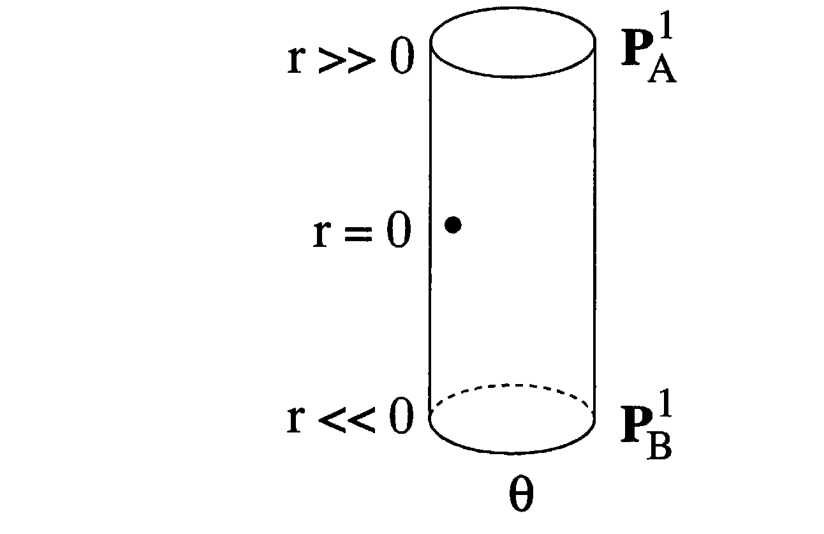
\includegraphics[width=0.40\textwidth]{figs/fig_p187_1.png}
  \caption{与 Figure 3 同构的参数柱面：$r\gg0$ 处靶空间为 $\mathbf{P}^{1}_{A}$ 上的 $\mathcal{O}(-1)\oplus\mathcal{O}(-1)$，$r\ll0$ 处为 $\mathbf{P}^{1}_{B}$ 上的同一丛，黑点标出 $r=0$ 处的奇点，水平方向为 $\theta$。（原文 Figure 4，p.187）}
  \label{fig:p187-1}
\end{figure}

更一般地，考虑两个双有理等价的 Calabi–Yau 流形 $X$ 与 $X'$，其等价方式使得它们的丰富锥（ample cone）彼此相接。

\begin{figure}[htbp]
  \centering
  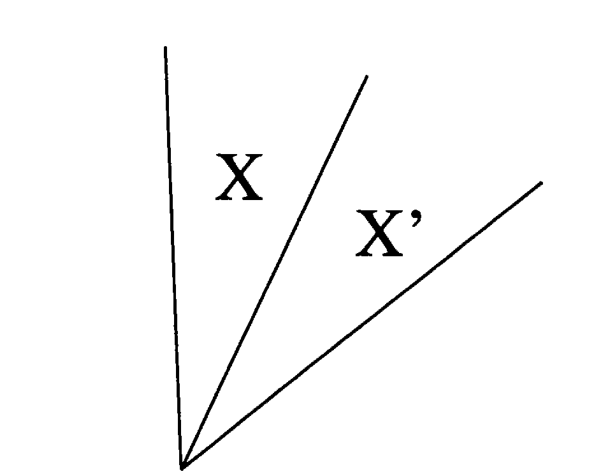
\includegraphics[width=0.36\textwidth]{figs/fig_p187_2.png}
  \caption{两个双有理等价的 Calabi–Yau 流形 $X$ 与 $X'$ 的 Kähler 锥沿一条公共的壁相接，图中以三条自原点出发的射线表示锥的边界。（原文 Figure 5，p.187）}
  \label{fig:p187-2}
\end{figure}

为简单起见设 $h^{2,0}=0$，并注意双有理变换不会改变 $h^{p,0}$ 的值。经典地，要从 $X$ 走到 $X'$，必须经过 Kähler 锥壁上的一个奇点。这个奇点与我们在“flop”例子中于 $r=0$ 处刚发现的奇点颇为相似。在量子场论中，人们可以取 $\theta\ne0$ 绕过这个奇点；于是只要变动共形场论的参数，就能从 $X$ 光滑地延拓到 $X'$。

% [Tutor Note: 这个“flop”例子其实就是 conifold（锥形奇点）：$\mathbb{C}^{4}$ 在 $\mathbb{C}^{*}$ 的权 $(1,1,-1,-1)$ 作用下的两个 GIT 商，正是 conifold 的两个“小解消” $\mathcal{O}(-1)\oplus\mathcal{O}(-1)\to\mathbf{P}^{1}$，而 flop 就是连接二者的双有理变换。两侧都是 $h^{1,1}=1$、$h^{2,1}=0$，且 $h^{p,0}$ 在 flop 下不变，这与正文“双有理变换不改变 $h^{p,0}$”相符（一般 flop 会使 $h^{1,1}$ 改变 $\pm1$、$h^{2,1}$ 反向改变而 Euler 数不变；本例中两个小解消同构，故 Hodge 数完全不变）。经典几何必须穿过 conifold 奇点，量子场论则借 $\theta\ne0$ 绕过——这是“量子几何把经典上必须退化的模空间光滑地连起来”的典型例子。另外，“$h^{2,0}=0$”对 Calabi–Yau 三维复流形（threefold）本已自动成立，作者写下它是为了排除由 $h^{2,0}$ 型周期（$B$ 场）带来的额外参数，使复化 Kähler 模空间成为唯一相关的模空间。]
